%\documentclass[german, twoside, parskip]{VRThesis} % dies ist eine deutsche Abschlussarbeit
\documentclass[twoside, parskip]{VRThesis} % this is an english bachelor/master thesis

% replace this by the title of the thesis
\title{Pre-operative Planning in Virtual Reality with Head Mounted Displays for Oral and Maxillofacial Surgery}
% replace this by the authors name
\author{Filip Kajzer}
% replace this by the date of issue (Abgabedatum), for PhD thesis date of the exam
\date{\today}                 

% options for master thesis and Diplomarbeit
% Matrikelnummer, student ID
\studentid{380 428}
\fieldofstudy{Informatik}
%\fieldofstudy{Software Systems Engineering}
\firstsupervisor{Prof. Dr. Torsten W. Kuhlen \\ Visual Computing Institute, University RWTH Aachen}
%\firstsupervisor{Prof. C. Bischof, Ph.D. \\ Institute for Scientific Computing}
\secondsupervisor{PD Dr. Dr. A. Modabber, MBA \\ Department for Oral and Maxillofacial Surgery, University Hospital RWTH Aachen}
\tutor{Andrea Bönsch, Behrus Puladi}

\addtolength{\oddsidemargin}{+.2in}
\addtolength{\evensidemargin}{-.2in}

\usepackage{enumitem}
\setlist[itemize]{noitemsep}

\begin{document} 

%\maketitle
%\makecoverMaster % this is the thesis cover (a shorter version of the title page)
%\maketitleMaster % this is the thesis title page

% generates the statement (Erkl�rung) page for master thesis and Diplomarbeit
%\makestatement

% generates the table of contents (Inhaltsverzeichnis)
\tableofcontents

\chapter{Introduction}

This master thesis is in context of a cooperation between the Visual Computing Institute at RWTH Aachen University and the Department of Oral and Maxillofacial Surgery (OMFS) at University Hospital RWTH Aachen (UHA).
The goal of this thesis is to simulate a virtual operating room for oral and maxillofacial surgeons in Virtual Reality (VR).
Workflows and procedures will be strongly oriented towards clinical practices of the oral and maxillofacial department in UHA.

Through the well established field of medical imaging, surgeons can get a very detailed view of patient’s specific anatomy and pathology today. 
It is an essential part of preparing for surgery.
Most common medical 3D image acquisition techniques (not exlusive) are computed tomography (CT), cone-beam computed tomography (CBCT) and magnetic resonance imaging (MRI).
CT / CBCT makes use of x-ray measurements from different angles to produce cross-sectional (tomographic) "slices" of the scanned site.
With this technique, bone structure and soft tissue can be displayed in medical imaging.
The disadvantage of these techniques is the exposure to carcinogenic x-rays.
In MRI, strong magnetic fields, magnetic field gradients and ultrasound are used to create tomography of the patients tissue.
Since this technique makes use of hydrogen atoms, which is predominantly present in patient's soft tissue, bone structure is not imaged well.
However, when studying mandibular joints for example, MRI is able to outperform CT \cite{RN65}.
The most recent one, CBCT, lowers radiation dosage of traditional CT and continually contributes to the accuracy of diagnostic tasks of the viscerocranium.
It is able to produce images with isotropic submillimeter spatial resolution, which is ideally suited for isolated viscerocranium scans. 
The radiation dosage of CBCT is less than traditional CT and thus helps optimize health-to-risk ratio \cite{WHITE2008689}.

As discussed, there are a variety of ways to acquire medical imaging.
However, the displaying methods of 3D medical imaging data is very limited for clinicians.
After acquiring raw data via mentioned techniques, volume images are generated. 
Generally, data is reconstruced in three planes (axial, sagittal and coronal).
Each plane is represented in "slices" which are 2D images of the volume image in an axis.
The distance between each slice can differ but is usually between one and five millimeters.

OMFS is very diverse. It has to handle a complex arrangement of bones, teeth, vessels, cartilage, nerves, muscles, skin and gland tissue.
These structures can be deeply complex, even more so in the viscerocranium.
Therefore, OMF surgeons rely heavily on accurate 3D medical imaging to plan procedures.
Even though three-dimensional objects are being analysed and also generated, they are viewed in a two-dimensional format on conventional computer screens.
The generated slices from medical imaging are viewed in the mentioned planes to get volumentric understanding of patient's underlying anatomy and pathology.
The problem with slices is that they are generally unsegmented and it is up to the viewer of the medical imaging to interpret them correctly.

To prepare for medical procedures, a number of preparational options are at the surgeons disposal.
Each of those common practices will be discussed based on how well it is suited for the individuality of patients, the realism and the cost (time and resources) associated with preparing for the operation.

The most common preparation technique is the mental simulation in which the surgeon uses his imagination to get a mental image of the surgical site.
This is solely dependant on the experience and spatial imagination of the surgeon. 
Hence it can be very patient specific, which is the goal in such an excercise.
The realism however is low to medium and the costs are also dependant on the expercience and skill of the surgeon himself.

Another, yet very costly technique is a simulation on 3D-printed models.
Since patient data is used here, it is an highly patient specific and highly realistic simulation.

In papersimulations, surgeons draw out treatment plans.
This is usually little patient specific and not realistic, however the costs are very low too.

The last technique presented are operational textbooks and videos.
They are not patient specific at all, but due to real operations being depicted the realism is generally low to medium.
The cost is also almost zero since the hospital will generally own a number of textbooks and videos for training.

Each of theses techniques has major disadvantages.
They all cannot actively reflect the underlying specific anatomy and pathology of the patient and lack spatial perception.
Also, the 3D medical imaging, which gets viewed on 2D computer screens, has to be translated back onto the patient via the surgeons imaginative power. 
As discussed, there does not seem to be a trivial technique which all surgeons should use.
Surgeons will often use a combination of mentioned techniques to get the best results.
In the preparation stage, it is crucial that the operator gets a well defined mental image by 3D medical imaging data of the patient's anatomy and pathology.

This thesis aims to improve medical imaging and pre-operational planning by using a modern approach with head-mounted displays.
By using acquired 3D medical imaging in a virtual reality application, a very patient specific, highly realistic and only moderately costly technique with which surgeons can prepare for operations is pursued.

This thesis aims to achieve the following advantages over conventional methods:
\begin{compactenum}[label=(\alph*)]
    \item Familiarize the operator with the patient specific anatomy and pathalogy before operating
    \item The ability to simulate important operation steps
    \item Allow revision of the virtual operation as often as needed
    \item Recording and analysis of users and others virtual operations
    \item Test out procedures
\end{compactenum}

Especially the imaging of voluminous objects is mentally demanding and this thesis hopes to eliminate this problem completely by providing realistic 3D medical imaging in virtual reality.
This thesis is part of an applied virtual and augmented reality workflow for oral and maxillofacial surgery using head mounted displays (HMDs) as described in Figure \ref{fig::ProjectPlan}.

\begin{figure}[ht!]
    \centering
    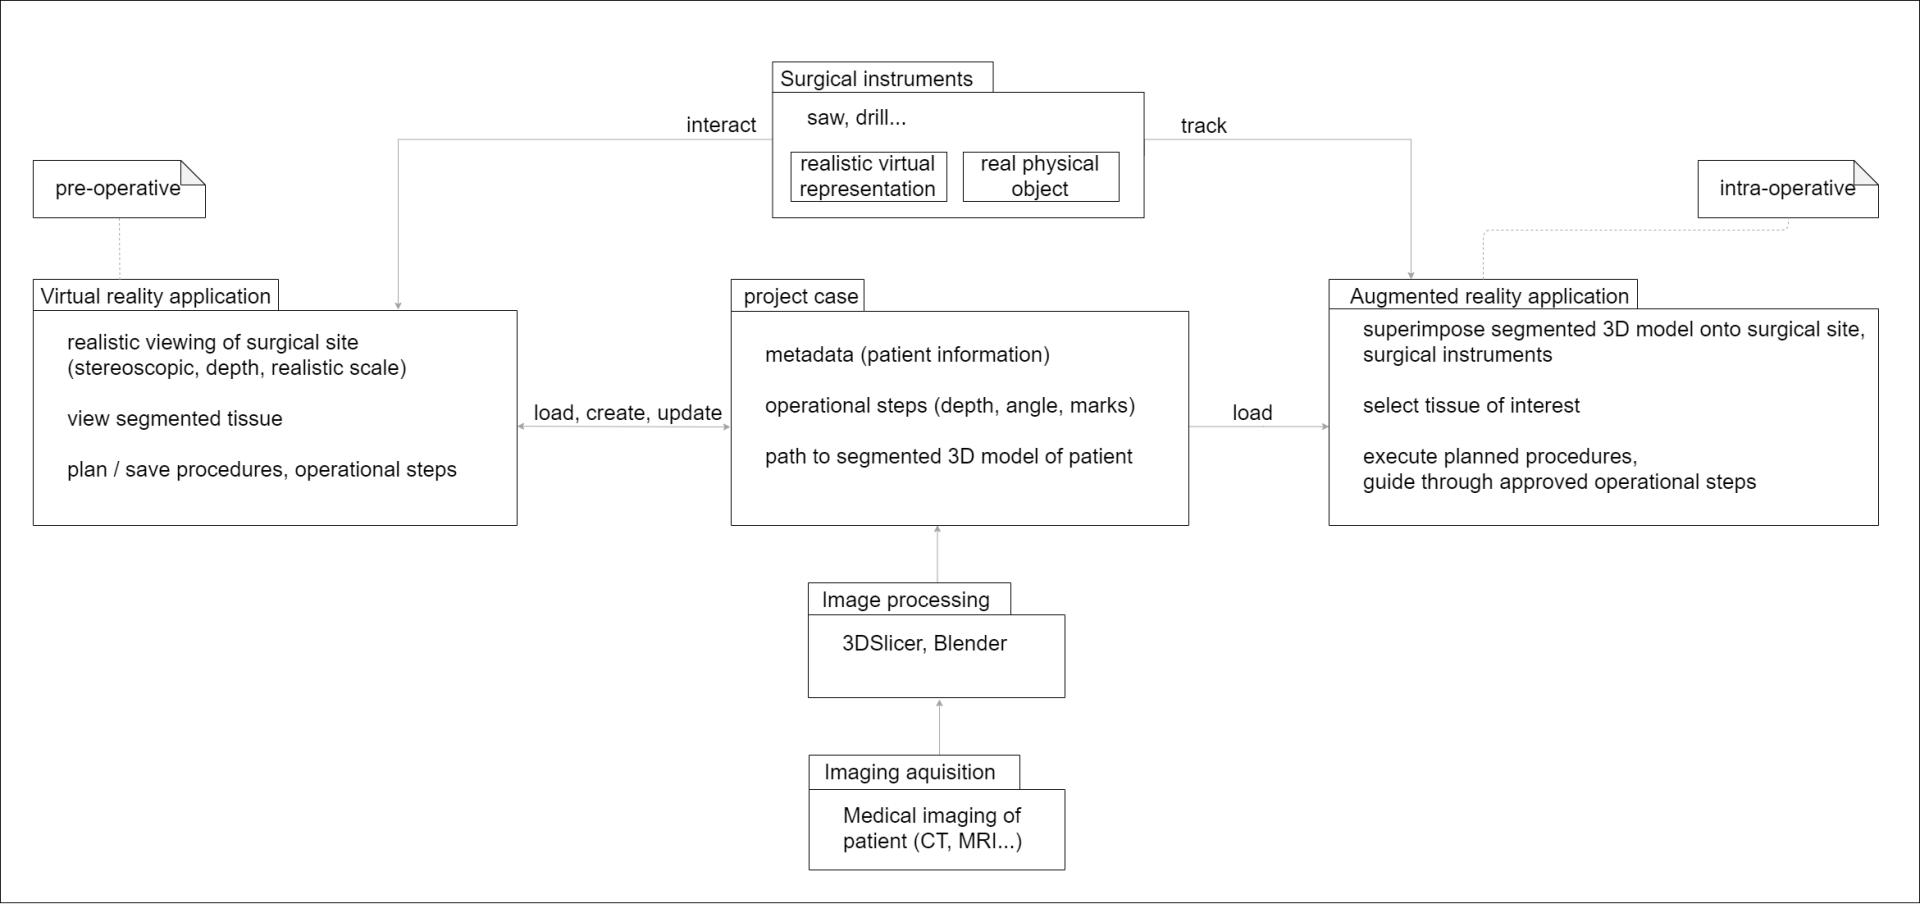
\includegraphics[width=\linewidth]{images/project_plan.png}
    \caption{\label{fig::ProjectPlan} Complete VR and AR workflow for surgeons concept}
\end{figure}

The main goal of this thesis is to create a pre-operative assistance tool in VR with HMDs for oral and maxillofacial surgery as highlighted in Figure \ref{fig::ProjectPlan}. 
In addition, the results of the pre-operative planning might be used intra-operatively to provide assistance via Augmented Reality (AR) as described in the workflow.
To provide a useful preparational tool, it is critical to simulate individual operation steps.
Planned steps will be storable in a format in which they can be loaded and viewed in both the virtual and augmented reality applications bi-directionally as described.
By planning the operational steps in virtual reality, planned procedures can easily be shown to other staff involved.
Naturally, it will be of uttermost importance that we have medical equipment and an appropriate virtual environment recreated remarkably close to reality.

The remainder of this Exposé is structured as follows: Chapter 2 provides a brief overview of related endevours made in the medical field.
Chapter 3 gives a scope of the thesis and a broad monthly schedule.

\chapter{Related Work}

A key part of this thesis is to advance the area of visualisation of medical imaging.
Even though techniques exist, operations are still planned on two-dimensional images for three-dimensional surgical sites.
In 2009, Swennen et al. discuss several improvements for three-dimensional treatment planning over conventional methods \cite{swennen2009three}.
Cost reduction and better patient outcome were achieved with three-dimenstional treatment planning, even though the planning was still conducted on conventional computers with 2D screens.
Especially the diagnosis, treatment planning and treatment communication were improved.
Additionally, experts all over the world can be consulted since treatment plans can be send via electronic mail.
As VR technology advances and entry costs are reduced, VR is considered more and more for a wide spectrum of applications.
In surgery, the main focus of research is on surgical training with pre-modeled patient anatomy and pathology.
By using state-of-the-art medical imaging and virtual reality technology and head mounted displays, this thesis aims to advance medical visualisation and surgery planning for patient specific procedures.
In Section \ref{sec::RelatedWork1}, we will take a look at efforts made in creating a low cost surgical simulation to train novice surgeons.
The simulator aims to create pre-trained novices for cervical cancer surgery. 
Cervical cancer is one of the world's leading causes of death \cite{RN52}.
By developing low-cost systems and using commercially available technologies, costs can be reduced significantly over traditional training.
This is crucial for resource-challenged countries, where the main benefit of low cost VR surgery simulations is predicted.
In Section \ref{sec::RelatedWork2}, the OMFS specific training tool "VR Surgery" will be presented.
VR Surgery was developed as a visualisation aid for senior surgeons and as a practice tool for novices.   

\section{\label{sec::RelatedWork1}Creating a low-cost virtual reality surgical simulation to increase surgical oncology capacity and capability}
Worldwide, less than 25 percent of people with cancer requiring surgery have access to safe, affordable and timely surgery \cite{RN52}.
One way of increasing the surgical capacity is to reduce time and cost of training novices.
Parham et. al (2019) present a novel approach for training novice surgeons \cite{RN52}.
By developing a low cost simulation, using commercially available VR software and the Oculus Rift HMD, they have succesfully 
helped surgeons to prepare for radical abdominal hysterectomy surgery procedures.
A near identical representation of an operating theatre using 1:1 scale was used for immersion.
3D replica of human female pelvic anatomy and pathalogy including organs, veins, peritoneum and connective tissue was created.
A huge focus while developing was to simulate reality as accurately as possible. 
Immersing trainees in the simulator is crucial so that they can focus on learning and practise without distractions.
Putting them in a realistic operating scenario helps reducing anxiety and selfconsciousness before first time operations \cite{RN52}.

Parham et. al recognize a need for clinical testing to establish VR efficacy, since there is a lack of research for VRs clinical utility \cite{RN59}. 
However, VR was already considered over 10 years ago as an important addition to surgical training, with a prediction for even more relevance in the future \cite{RN60}.
These low cost VR applications could be especially considered for resource-challenged countries where there is a lack of skilled workforce, mainly because of cost.

This simulator creates pre-trained novices by providing new ways to acquire the psycho-motor skills, sensory acuity and cognitive planning abilities needed for sugery.
Virtual reality based training is already proven to reduce the time to acquire surgical proficiency \cite{RN61,RN62}. 
In randomized control studies, VR trained trainees performing laparoscopic cholecystectomy, made fewer errors and were faster \cite{RN63,RN64}.
VR trained trainees required only half the time to reach the skill level of intermediately skilled surgeons compared to standard training.
Hence, it is proven that skills acquired in simulations can successfully be translated to the operting theatre (OT) \cite{RN63,RN64}.

Parham et. al focus on high-quality visuals for immersion.
All assets are represented in 1:1 scale and the correct visual reproduction of organs, tools and hand positions is ensured through thorough analysis of real world counterparts.
Object materials are physics-based and organic materials approximated by an physics engine.
The lighting emerging from medical equipment is based on their specifications.
Lastly, the software would be developed with future expansion into other medical fields in mind \cite{RN52}.

The virtual OT consists of the open surgical area including organs of the patient, a tray for surgical instruments and a monitor displaying simulated patient vitals and procedure instructions.
It was modeled after a real world OT located inside the University Teaching Hospital in Lusaka, Zambia.
The assets were modeled after recieving reference photos and videos of locations and instruments and researching the female anatomy.
It was argued that even though 3D scans of real human organs exists, they are too inefficient to run in real time VR \cite{RN52}.

In the virtual reality simulation, the trainee stands in the virtual OT with an operating table, tray of surgical instruments and the surgery awaiting patient with cervical cancer.
The procedure is closely modeled after an actual surgical procedure, meaning the surgical site is exposed while the rest of the patient is covered.
Instructions are given via a monitor above the operating table and audio feedback is given to guide the trainee through the simulation.
The simulation lasts roughly 20 minutes and provides feedback on the trainees accuracy on various postions of the procedure and an overall score.
To compare traditional surgical training versus VR, the trainees are assessed by expert surgeon-mentors \cite{RN52}.

It is mentioned how commercial VR will advance significantly in the future, allowing for an even better adoption of VR simulations in surgery.
Surgical training enhanced with augmented and virtual reality will have wide applications according to Parham et. al.
However, such technology has to be carefully build and clinically tested.
VR and AR has the potential to help train the workforce and to ensure higher quality standards \cite{RN52}.

The goal of this thesis is to apply virtual reality in oral and maxillofacial surgery treatment planning.
In contrast to the presented work, this thesis aims to provide a useful tool not only for learning, but also for planning patient specific surgery.
Because of technology advancing rapidly, VR and AR become more and more affordable options.
Mentioned limitations for patient specific 3D models are not an issue anymore.
By using patient anatomy and pathology specific models, surgeons can profit from the mentioned benefits of VR simulation not only as a learning tool.
Moreover, the goal is to give trained surgeons a useful tool which adds to the arsenal of existing planning techniques.
However, trainees can also benefit immensely by studying and reproducing planned procedures of experts.
Another aspect of VR is the ability to communicate on a global level. 
In fields where expects are rare, planned procedures by such experts could be viewed and studied to get greater insight.


\section{\label{sec::RelatedWork2}VR Surgery: Interactive Virtual Reality Application for Training Oral and Maxillofacial Surgeons using Oculus Rift and Leap Motion}
Worldwide, less than 25 percent of people with cancer requiring surgery have access to safe, affordable and timely surgery \cite{RN52}.
One way of increasing the surgical capacity is to reduce time and cost of training novices.
Parham et. al (2019) present a novel approach for training novice surgeons \cite{RN52}.
By developing a low cost simulation, using commercially available VR software and the Oculus Rift HMD, they have succesfully 
helped surgeons to prepare for radical abdominal hysterectomy surgery procedures.
A near identical representation of an operating theatre using 1:1 scale was used for immersion.
3D replica of human female pelvic anatomy and pathalogy including organs, veins, peritoneum and connective tissue was created.
A huge focus while developing was to simulate reality as accurately as possible. 
Immersing trainees in the simulator is crucial so that they can focus on learning and practise without distractions.
Putting them in a realistic operating scenario helps reducing anxiety and selfconsciousness before first time operations \cite{RN52}.

Parham et. al recognize a need for clinical testing to establish VR efficacy, since there is a lack of research for VRs clinical utility \cite{RN59}. 
However, VR was already considered over 10 years ago as an important addition to surgical training, with a prediction for even more relevance in the future \cite{RN60}.
These low cost VR applications could be especially considered for resource-challenged countries where there is a lack of skilled workforce, mainly because of cost.

This simulator creates pre-trained novices by providing new ways to acquire the psycho-motor skills, sensory acuity and cognitive planning abilities needed for sugery.
Virtual reality based training is already proven to reduce the time to acquire surgical proficiency \cite{RN61,RN62}. 
In randomized control studies, VR trained trainees performing laparoscopic cholecystectomy, made fewer errors and were faster \cite{RN63,RN64}.
VR trained trainees required only half the time to reach the skill level of intermediately skilled surgeons compared to standard training.
Hence, it is proven that skills acquired in simulations can successfully be translated to the operting theatre (OT) \cite{RN63,RN64}.

Parham et. al focus on high-quality visuals for immersion.
All assets are represented in 1:1 scale and the correct visual reproduction of organs, tools and hand positions is ensured through thorough analysis of real world counterparts.
Object materials are physics-based and organic materials approximated by an physics engine.
The lighting emerging from medical equipment is based on their specifications.
Lastly, the software would be developed with future expansion into other medical fields in mind \cite{RN52}.

The virtual OT consists of the open surgical area including organs of the patient, a tray for surgical instruments and a monitor displaying simulated patient vitals and procedure instructions.
It was modeled after a real world OT located inside the University Teaching Hospital in Lusaka, Zambia.
The assets were modeled after recieving reference photos and videos of locations and instruments and researching the female anatomy.
It was argued that even though 3D scans of real human organs exists, they are too inefficient to run in real time VR \cite{RN52}.

In the virtual reality simulation, the trainee stands in the virtual OT with an operating table, tray of surgical instruments and the surgery awaiting patient with cervical cancer.
The procedure is closely modeled after an actual surgical procedure, meaning the surgical site is exposed while the rest of the patient is covered.
Instructions are given via a monitor above the operating table and audio feedback is given to guide the trainee through the simulation.
The simulation lasts roughly 20 minutes and provides feedback on the trainees accuracy on various postions of the procedure and an overall score.
To compare traditional surgical training versus VR, the trainees are assessed by expert surgeon-mentors \cite{RN52}.

It is mentioned how commercial VR will advance significantly in the future, allowing for an even better adoption of VR simulations in surgery.
Surgical training enhanced with augmented and virtual reality will have wide applications according to Parham et. al.
However, such technology has to be carefully build and clinically tested.
VR and AR has the potential to help train the workforce and to ensure higher quality standards \cite{RN52}.

The goal of this thesis is to apply virtual reality in oral and maxillofacial surgery treatment planning.
In contrast to the presented work, this thesis aims to provide a useful tool not only for learning, but also for planning patient specific surgery.
Because of technology advancing rapidly, VR and AR become more and more affordable options.
Mentioned limitations for patient specific 3D models are not an issue anymore.
By using patient anatomy and pathology specific models, surgeons can profit from the mentioned benefits of VR simulation not only as a learning tool.
Moreover, the goal is to give trained surgeons a useful tool which adds to the arsenal of existing planning techniques.
However, trainees can also benefit immensely by studying and reproducing planned procedures of experts.
Another aspect of VR is the ability to communicate on a global level. 
In fields where expects are rare, planned procedures by such experts could be viewed and studied to get greater insight.


\chapter{Scope of the Thesis}

This chapter outlines the requirements of this thesis based on the challenges mentioned in Chapter 1.
It will also outline a broad monthly schedule of the thesis at the end.
As this thesis is part of a greater workflow, we will also clarify in which way the software components need to communicate and how it will be implemented.

\section{\label{sec::Features}Features of the Virtual Reality Application}
As this thesis is a completely new project we will need to build an architecture from the ground up.
Since the main focus of this thesis is visualisation and planning, we aim to provide a realistic feeling experience without being unnecessarily complex.
This means that while our main goal is surgery simulation, we do not focus on realistic physical behaviour of tissue.
The following anonymous, randomly selected data will be provided by the department of oral and maxillofacial surgery in the university hospital of the RWTH Aachen:
\begin{compactenum}[label=(\alph*)]
    \item Imaging acquisition
    \begin{compactenum}[label=(\alph*)]
        \item CT/CBCT scans, MRI scans
        \item provided by the UHA
    \end{compactenum}
\item Image processing
    \begin{compactenum}[label=(\alph*)]
        \item Apply techniques to segment tissue from scans
        \item Create three-dimensional objects from segmented data
        \item Export data into conventional three-dimensional objects which can be used in the application
    \end{compactenum}
\end{compactenum}

Furthermore, following key components will be designed and developed for this thesis to give an immersive experience:

\begin{compactenum}[label=(\alph*)]
    \item Virtual operating room
        \begin{compactenum}[label=(\alph*)]
            \item Based on real locations in the UHA
            \item If possible, designed via photogrammetry
        \end{compactenum}
    \item Provide an interaction system where the user can:
        \begin{compactenum}[label=(\alph*)]
            \item Freely move around
            \item Interact with virtual model of patient:
                \begin{compactenum}[label=(\alph*)]
                    \item Magnify and reset to original
                    \item Project another copy of the initial model for comparison
                    \item Set cutting planes
                    \item Mirror at symmetry line
                    \item Simulate cuts including depth by drawing
                    \item Measuring of the following attributes:
                        \begin{compactenum}[label=(\alph*)]
                            \item distance between two points
                            \item surface / volume area
                            \item angle
                        \end{compactenum}
                    \item Transparancy slider for segmented tissue
                    \item Select which tissue to view
                \end{compactenum}
            \item Grab surgical instruments
            \item Use instruments for intended operational procedures (drilling, sawing etc.)
            \item Start, undo, save recording movements of currently selected instrument 
            \item Start screen capture (Photo, Video)
        \end{compactenum}
    \item Surgical Instruments and materials
        \begin{compactenum}[label=(\alph*)]
            \item Create realistic virtual objects from real physical instruments and materials which are used in the oral and maxillofacial department of the UHA
            \item Mechanism to plan and view procedures in relation to the patient including:          
                \begin{compactenum}[label=(\alph*)]
                    \item Angle of the instrument
                    \item Movements including direction of the instrument
                    \item Depth of the instrument if patient was penetrated
                    \item Markings on the patient
                    \item Inform if critical tissue was penetrated
                \end{compactenum}
            \item Mechanism to start, stop, redo recordings of procedures for each instrument
        \end{compactenum}
    \item Provide an interface to the augmented reality application:
        \begin{compactenum}[label=(\alph*)]
            \item The user should be able to view all necessary patient data
            \item The user should be able to view screen captures
            \item The user should be able to load planned procedures in both applications by using an agreed format
        \end{compactenum}
\end{compactenum}

The software will be developed with commercially available hard- and software.
The HMD in which this software will be developed is the HTC Vive.
As user input, the Valve Index controller will be used.
The software will be developed in Unity (LTS 2018.4) using the SteamVR (2.0) interaction system in the C\# programming language.
Since running virtual reality software is computationally expensive, a desktop pc with the following hardware is recommended for highest immersion:

\begin{compactenum}[label=(\alph*)]
    \item Graphics Card: Nvidia GTX 1060 or equivalent
    \item CPU: Intel i5-4590 / AMD Ryzen5 1500X
    \item Memory (RAM): 8GB+
\end{compactenum}

The first step in realizing these requirements is to develop a software architecture with an interface to the augmented reality application in mind.
Since this is a bi-directional data exchange which does not need to be real time, one obvious approach would be to use a simple object notation language such as JSON.
A humanly readable format will be used so that operation plans can even be constructed without the need of an HMD.
Different options will be explored and decided upon in the beginning phase of the thesis.

After deciding on a software architecture, the next step is to create a virtual operating room and first surgical instruments.
The operation room will be designed after real operation rooms inside of the UHA.
A photogrammetry approach will be evaluated in the hope to give the most realistic experience as possible for OMF surgeons.
Virtual objects will be combined with a scan of the real world to give an interactive and immersive experience.
After the operating room, the focus will be on developing a traversing mechanism which allows for free exploration of the operating room.
Since operating rooms are not too large in general, it should be possible to traverse them in room-scale VR.
However, a teleport function will be added for convenience.
The surgical instruments will either be created in a 3D modelling software or exported in a similar way to how we obtain the segmented patient models from medical imaging.
The full functionality of the instruments will be developed in a later stage, since we will first work on the more important planning tools.

The planning tools will be the most critical part of the thesis, since they have to behave as expected.
There will be a mix of planning tools which are represented by virtual surgical instruments and basic features which will be mostly visualisation assistance.
At this stage, it will be crucial that the user inteface (UI) is as intuitive as possible and does not distract in any way.
Improving the UI however will be a continious effort throughout the thesis, and will hopefully become as intuitive and assisting as possible.

Each of the surgical instruments will have its own planning operations which can be recorded and saved.
Since at this stage, the architecture and format will already be decided, there should not be too much to worry about when implementing this feature.

There are currently no plans to hold a user study, however an expert review by working surgeons is planned to evaluate the usability and percieved realism of the tool.
Additionally, a small questionnaire will be used after surgery to determine if the new tool is preferred over conventional methods.

There are also possible optional features, such as an additional tool to view dicom data directly, which can be included in the scope of the thesis but will be decided upon during the development phase of the thesis and will be dependent on the progression of the core features of the tool.
As of now, a basic prototype is already developed to showcase some of the planned functionality of the application.






\section{Schedule}
The written part of the thesis will be worked on continuously throughout the whole six months period of the thesis, either in form of notes or directly written passages. What follows is a broad monthly schedule for the thesis:

\textbf{January:}
Designing a software architecture to allow the implementation of the requirements mentioned in Section \ref{sec::Features} and designing the structure of the "project cases" to save and load planned procedues.

\textbf{February:}
Start of the development phase of the thesis, beginning with implementing the a basic interaction system in which users can navigate and interact with objects.
This is important as a first step so that we can fully concentrate on the planning tools and the realistic operating room afterwards.

\textbf{March:}
Designing and implementing the virtual operating room and surgical instruments. Since an interaction system is already in place, the tools will already be interactable and base functionality provided.

\textbf{April / May:}
Implement planning operations (and save/load) and functionality for intended use of the surgical instruments (drill, saw...).
As mentioned in Section \ref{sec::Features}, it will be not important to have complex physics, but the necessary functionality of the instruments has to be implemented so that they are useful as planning tools.

\textbf{June:}
Finish the written part of the thesis.






\bibliography{ms_thesis,ms_endnote} 
\bibliographystyle{apalike}
%\bibliographystyle{ieeetr}

\end{document} 